%% talk_v5.tex — SHiP Timing Bar: END+TOP Hybrid Estimator
%% Author: René Ríos (ULS)
%% Compile: pdflatex -interaction=nonstopmode talk_v5.tex (×2)
\documentclass[aspectratio=169,9pt]{beamer}
\usetheme{Warsaw}
\usecolortheme{default}

%% Suppress Warsaw navigation balls (prevent headline overflow on many slides)
\setbeamertemplate{headline}{}
\setbeamertemplate{navigation symbols}{}

\usepackage[utf8]{inputenc}
\usepackage[T1]{fontenc}
\usepackage{amsmath,amssymb,booktabs,tabularx,colortbl}
\usepackage{tikz}
\usepackage{graphicx}

%% ── Author / title ──────────────────────────────────────────────────────────
\title[SHiP Timing Bar]{%
  SHiP Timing Bar:\\[4pt]
  END+TOP Hybrid T$_0$ Estimator\\[2pt]
  \small EJ-230 Scintillator, Vikuiti Reflector (R\,=\,0.95)}
\author{René Ríos}
\institute{Universidad de La Serena (ULS)}
\date{August 2026}

%% ── Colour macros (ROOT palette → xcolor) ──────────────────────────────────
\definecolor{cEnd}{RGB}{0,114,189}      % kAzure+2
\definecolor{cTop}{RGB}{217,118,25}     % kOrange+1
\definecolor{cBlu}{RGB}{0,128,0}        % kGreen+3
\definecolor{cOra}{RGB}{130,130,130}    % kGray+2
\definecolor{cRef}{RGB}{200,0,0}        % kRed+1

%% ── Convenience macros ──────────────────────────────────────────────────────
\newcommand{\sIQR}{\sigma_{\mathrm{IQR}}}
\newcommand{\sEnd}{\sigma_{\mathrm{END}}}
\newcommand{\sTop}{\sigma_{\mathrm{TOP}}}
\newcommand{\sBlu}{\sigma_{\mathrm{BLUE}}}
\newcommand{\veff}{v_{\mathrm{eff}}}
\newcommand{\Ntop}{N_{\mathrm{TOP}}}
\newcommand{\Npe}{N_{\mathrm{pe}}}
\newcommand{\Tze}{T_0^{\mathrm{END}}}
\newcommand{\Tzt}{T_0^{\mathrm{TOP}}}
\newcommand{\ps}{\ensuremath{\,\mathrm{ps}}}
\newcommand{\ns}{\ensuremath{\,\mathrm{ns}}}
\newcommand{\mm}{\ensuremath{\,\mathrm{mm}}}

% ─────────────────────────────────────────────────────────────────────────────
\begin{document}
% ─────────────────────────────────────────────────────────────────────────────

\begin{frame}
  \titlepage
\end{frame}

% ─────────────────────────────────────────────────────────────────────────────
\begin{frame}{Outline}
\tableofcontents
\end{frame}

% ─────────────────────────────────────────────────────────────────────────────
\section{Detector \& Simulation}

\begin{frame}{Timing bar geometry}
\begin{columns}[c]
\column{0.52\textwidth}
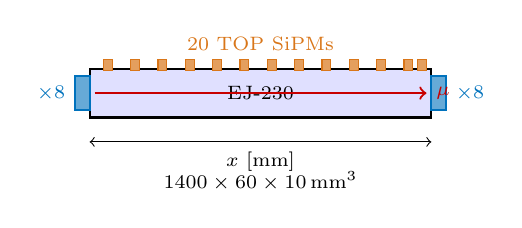
\begin{tikzpicture}[scale=0.62, every node/.style={font=\scriptsize}]
  % Bar body
  \filldraw[fill=blue!12,draw=black,thick]
    (0,0) rectangle (7,1.0);
  \node at (3.5,0.5) {EJ-230};
  % SiPMs on left end
  \filldraw[fill=cEnd!60,draw=cEnd,thick]
    (-0.3,0.15) rectangle (0,0.85);
  \node[left,cEnd] at (-0.3,0.5) {$\times8$};
  % SiPMs on right end
  \filldraw[fill=cEnd!60,draw=cEnd,thick]
    (7,0.15) rectangle (7.3,0.85);
  \node[right,cEnd] at (7.3,0.5) {$\times8$};
  % TOP SiPMs
  \foreach \xi in {0.28, 0.84, 1.40, 1.96, 2.52, 3.08, 3.64, 4.20,
                   4.76, 5.32, 5.88, 6.44, 6.72}{%
    \filldraw[fill=cTop!70,draw=cTop] (\xi,0.97) rectangle (\xi+0.18,1.18);
  }
  \node[above,cTop] at (3.5,1.18) {20 TOP SiPMs};
  % x arrow
  \draw[<->] (0,-0.50) -- (7,-0.50) node[midway,below] {$x$ [mm]};
  % beam arrow
  \draw[->,thick,cRef] (0.1,0.5) -- (6.9,0.5);
  \node[right,cRef] at (6.9,0.5) {$\mu$};
  % dimensions label
  \node[below=8pt] at (3.5,-0.45) {$1400 \times 60 \times 10\mm^3$};
\end{tikzpicture}

\vspace{4pt}
\begin{itemize}\setlength\itemsep{2pt}
  \item{\color{cEnd}\textbf{END}}: 2$\times$8 SiPMs on bar faces $\;\Rightarrow$ 16 channels
  \item{\color{cTop}\textbf{TOP}}: $\Ntop$ SiPMs on top surface
  \item Vikuiti ESR reflector on all lateral faces\\
    (dielectric–dielectric, $R=0.95$ constant)
\end{itemize}
\column{0.44\textwidth}
\begin{block}{Geant4 simulation}
\begin{itemize}\setlength\itemsep{2pt}
  \item Muons shot at 13 positions $x \in [-600,+600]\mm$
  \item 5000 events per position
  \item Branches: \texttt{event\_id, face\_type,}\\
        \texttt{time\_ns, pde, x\_mm, gun\_x\_mm}
  \item face\_type: 0=END-L, 1=END-R, 2=TOP
  \item SiPM: wavelength-dependent PDE
\end{itemize}
\end{block}

\begin{alertblock}{Material: EJ-230}
\footnotesize\centering
\begin{tabular}{ll}
Attenuation & $1200\mm$ \\
Decay time  & $1.5\ns$ \\
Rise time   & $0.5\ns$ \\
Yield & $9700\,\mathrm{MeV}^{-1}$ \\
$n$ & 1.58 \\
\end{tabular}
\end{alertblock}
\end{columns}
\end{frame}

% ─────────────────────────────────────────────────────────────────────────────
\begin{frame}{EJ-230 chosen for its fast decay — material comparison}
\begin{columns}[c]
\column{0.50\textwidth}
\centering
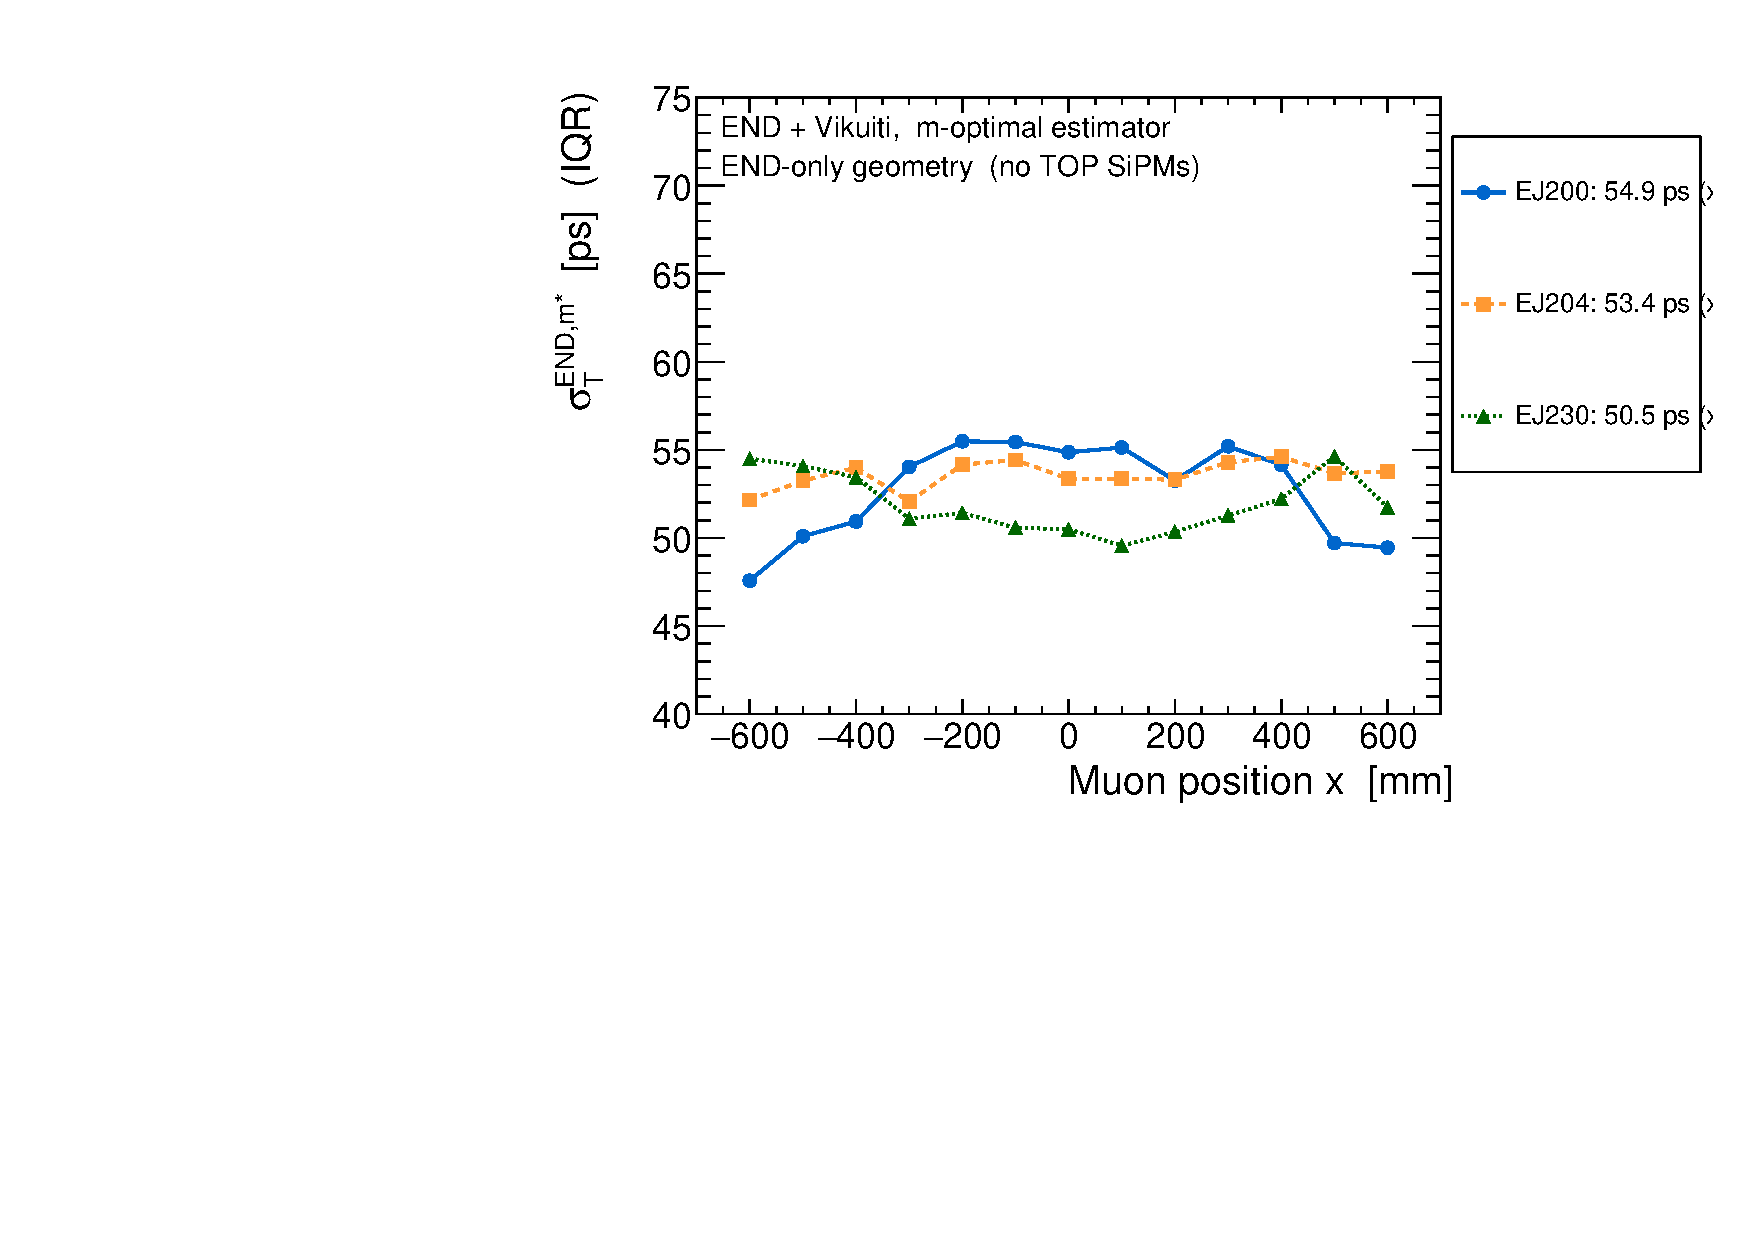
\includegraphics[width=\linewidth]{figs/figM1_mat_sigma_end.pdf}
\column{0.46\textwidth}
\begin{block}{Scintillator properties}
\scriptsize
\begin{tabular}{lccc}
\toprule
 & EJ-200 & EJ-204 & EJ-230 \\
\midrule
Att. [mm]     & 3800 & 1600 & \textbf{1200} \\
$\tau$ [ns]   & 2.1  & 1.8  & \textbf{1.5}  \\
$t_r$ [ns]    & 0.9  & 0.7  & \textbf{0.5}  \\
$Y$ [/MeV]    & 10000& 10400& 9700  \\
$n$           & 1.58 & 1.58 & 1.58  \\
\bottomrule
\end{tabular}
\end{block}
\begin{itemize}\setlength\itemsep{3pt}
  \item EJ-230: fastest rise ($t_r=0.5\ns$) and
    decay ($\tau=1.5\ns$)
  \item Shortest attenuation — photon loss toward
    center, but timing wins
  \item END-only at $x=0$: EJ-230 best despite
    fewer photons
  \item All three use $n=1.58$, $R=0.95$ reflector
\end{itemize}
\end{columns}
\end{frame}

% ─────────────────────────────────────────────────────────────────────────────
\section{Effective Velocity \& Nonlinearity}

\begin{frame}{Effective velocity from $\langle\Delta t\rangle$ vs $x$}
\begin{columns}[c]
\column{0.54\textwidth}
\centering
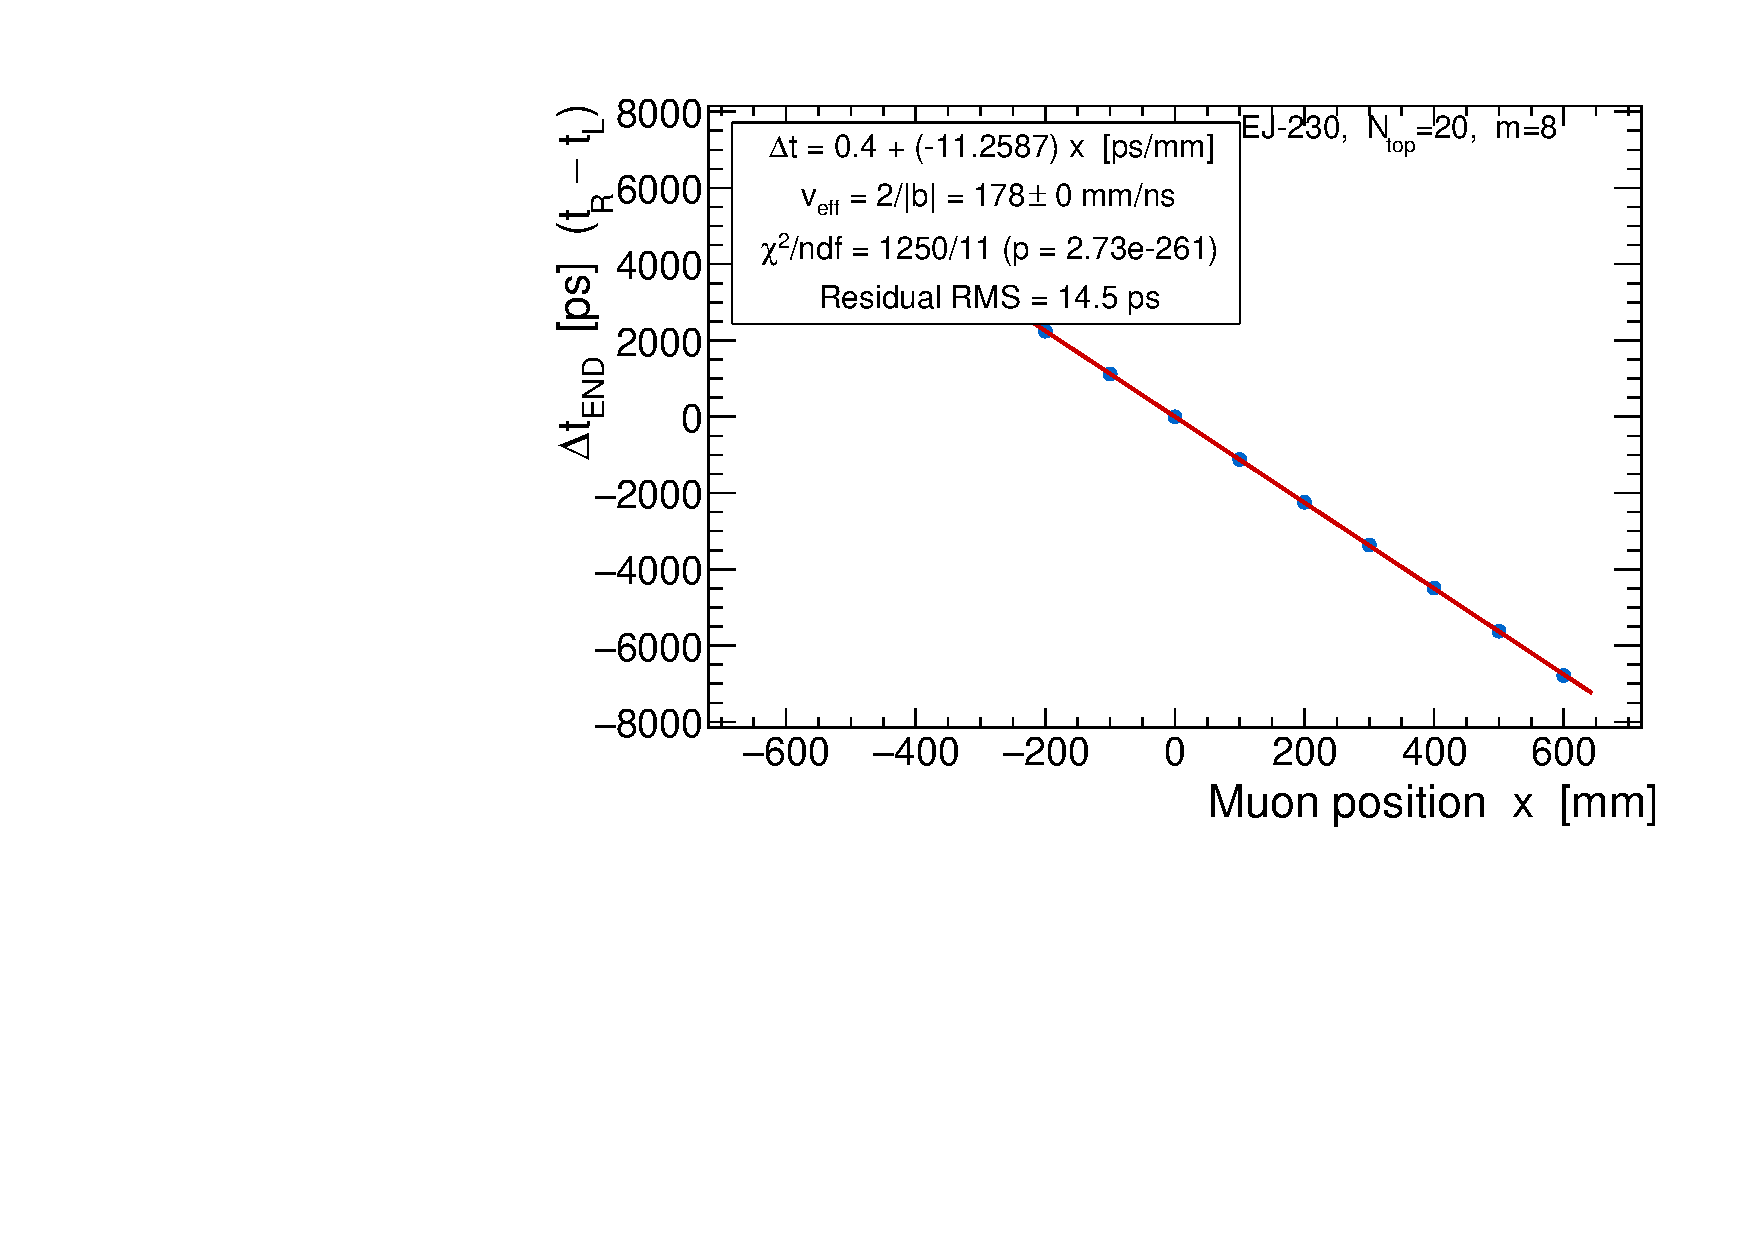
\includegraphics[width=\linewidth]{figs/v5_veff_fit.pdf}
\column{0.42\textwidth}
\begin{block}{Linear fit: $\Delta t = a + bx$}
\small
\begin{align*}
  b &= -11.259 \pm 0.001 \;\mathrm{ps/mm} \\
  \veff &= \frac{2}{|b|} = \mathbf{177.6 \pm 0.0\;\mathrm{mm/ns}} \\
  \chi^2/\mathrm{ndf} &= \mathbf{1250/11}
\end{align*}
\end{block}

\begin{alertblock}{Significant nonlinearity}
$\chi^2/\mathrm{ndf} = 1250/11$ is \emph{not} mild —
$p \approx 0$. The linear fit is a first-order
approximation; residuals shown next.
\end{alertblock}

\begin{itemize}\setlength\itemsep{2pt}
  \item Used: $m=8$ average estimator for $\Delta t$
  \item $\Delta t = t_R^{(m)} - t_L^{(m)}$
  \item Symmetry: $a \approx 0$ confirms bar
    is centred
\end{itemize}
\end{columns}
\end{frame}

% ─────────────────────────────────────────────────────────────────────────────
\begin{frame}{Nonlinearity residual has S-shape — edge photon loss}
\begin{columns}[c]
\column{0.52\textwidth}
\centering
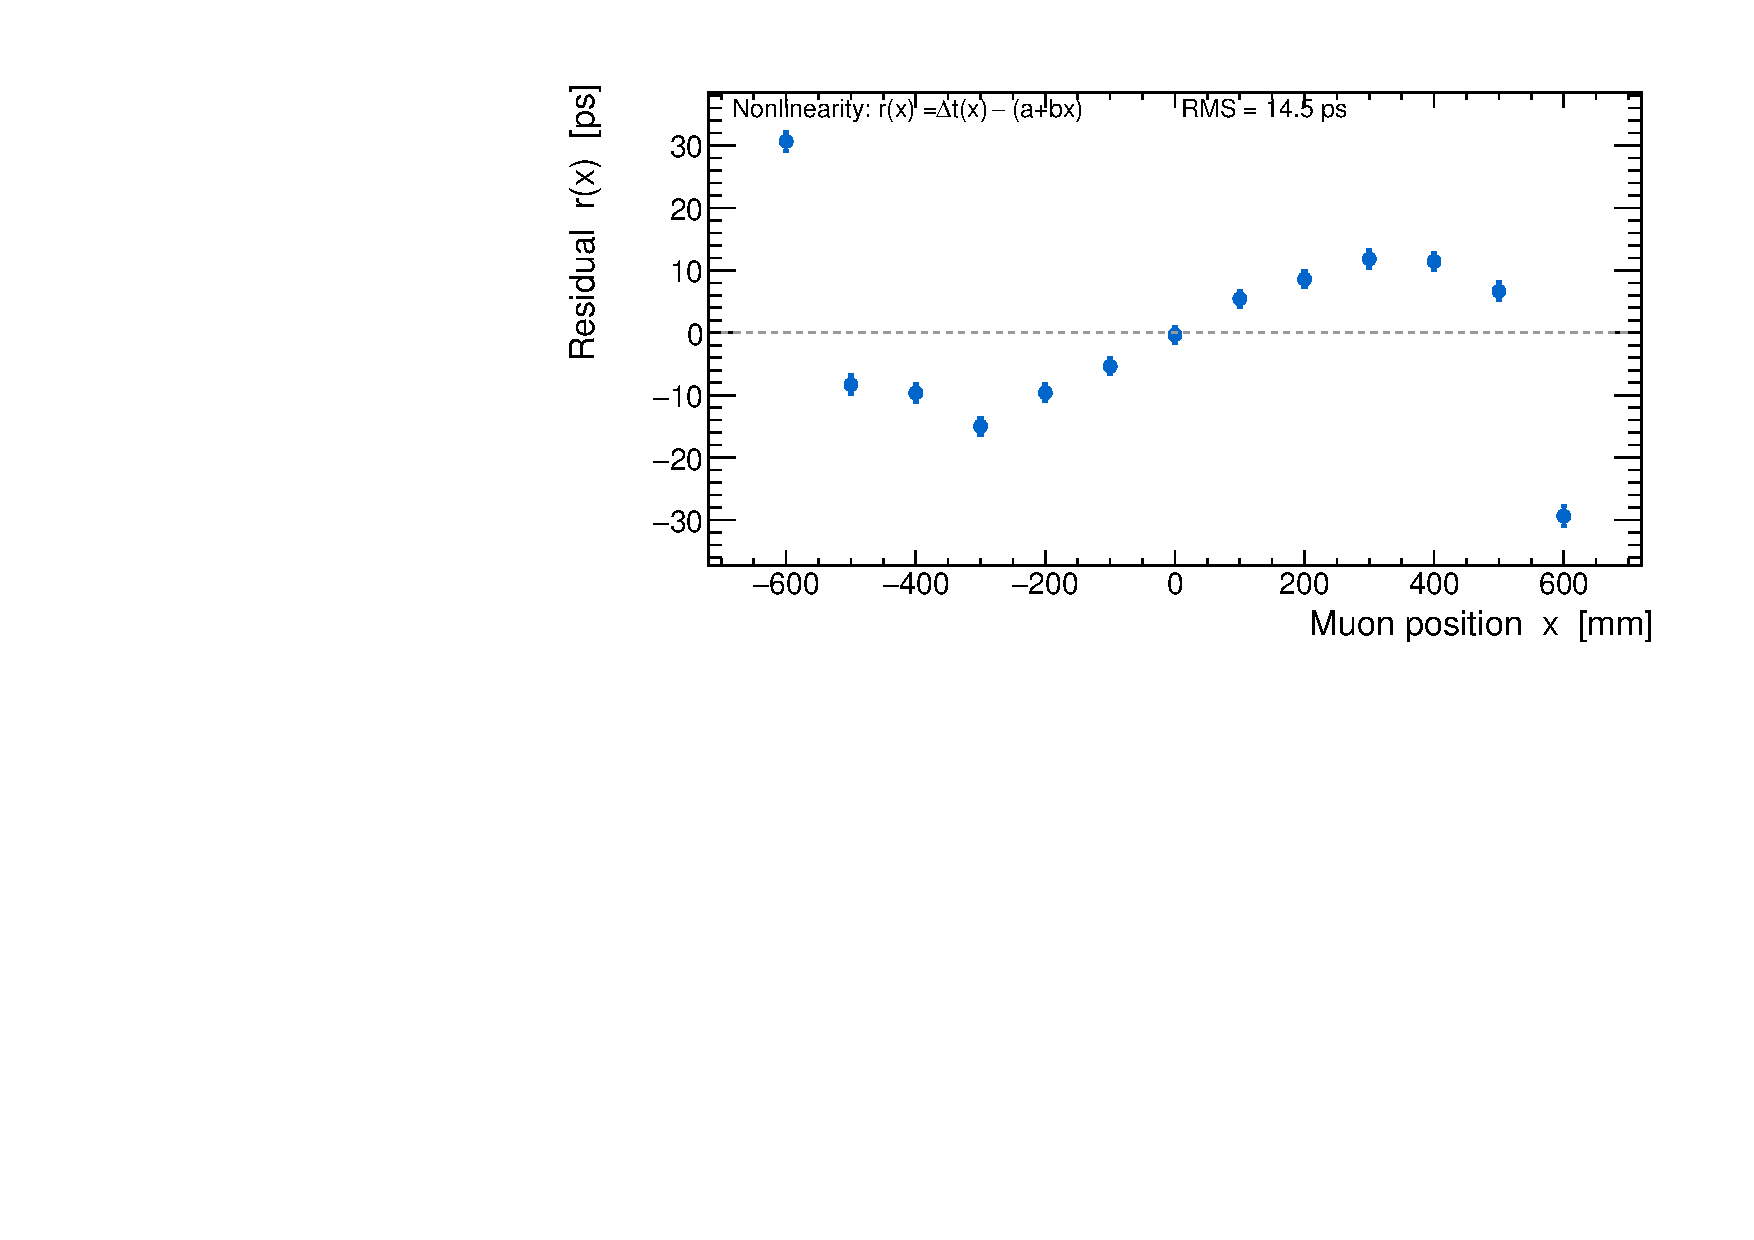
\includegraphics[width=\linewidth]{figs/v5_veff_residual.pdf}
\column{0.44\textwidth}
\begin{block}{Residual $r(x) = \langle\Delta t\rangle - (a+bx)$}
\small
RMS $= \mathbf{14.5\ps}$

\medskip
\scriptsize
\begin{tabular}{rr}
\toprule
$x$ [mm] & $r$ [ps] \\
\midrule
$-600$ & $+30.6$ \\
$-300$ & $-15.0$ \\
$\phantom{+}0$ & $-0.3$ \\
$+300$ & $+11.8$ \\
$+600$ & $-29.4$ \\
\bottomrule
\end{tabular}
\end{block}

\begin{itemize}\setlength\itemsep{3pt}
  \item S-shape: near $x=\pm600\mm$ photons
    arrive at the \emph{near} end first, biasing
    the average
  \item Residual RMS $\approx15\ps$ is the
    nonlinearity contribution to position bias
  \item For position reconstruction, a cubic
    correction should be applied
\end{itemize}
\end{columns}
\end{frame}

% ─────────────────────────────────────────────────────────────────────────────
\section{Timing Estimators}

\begin{frame}{END: $m$-average reduces jitter}
\begin{columns}[c]
\column{0.52\textwidth}
\centering
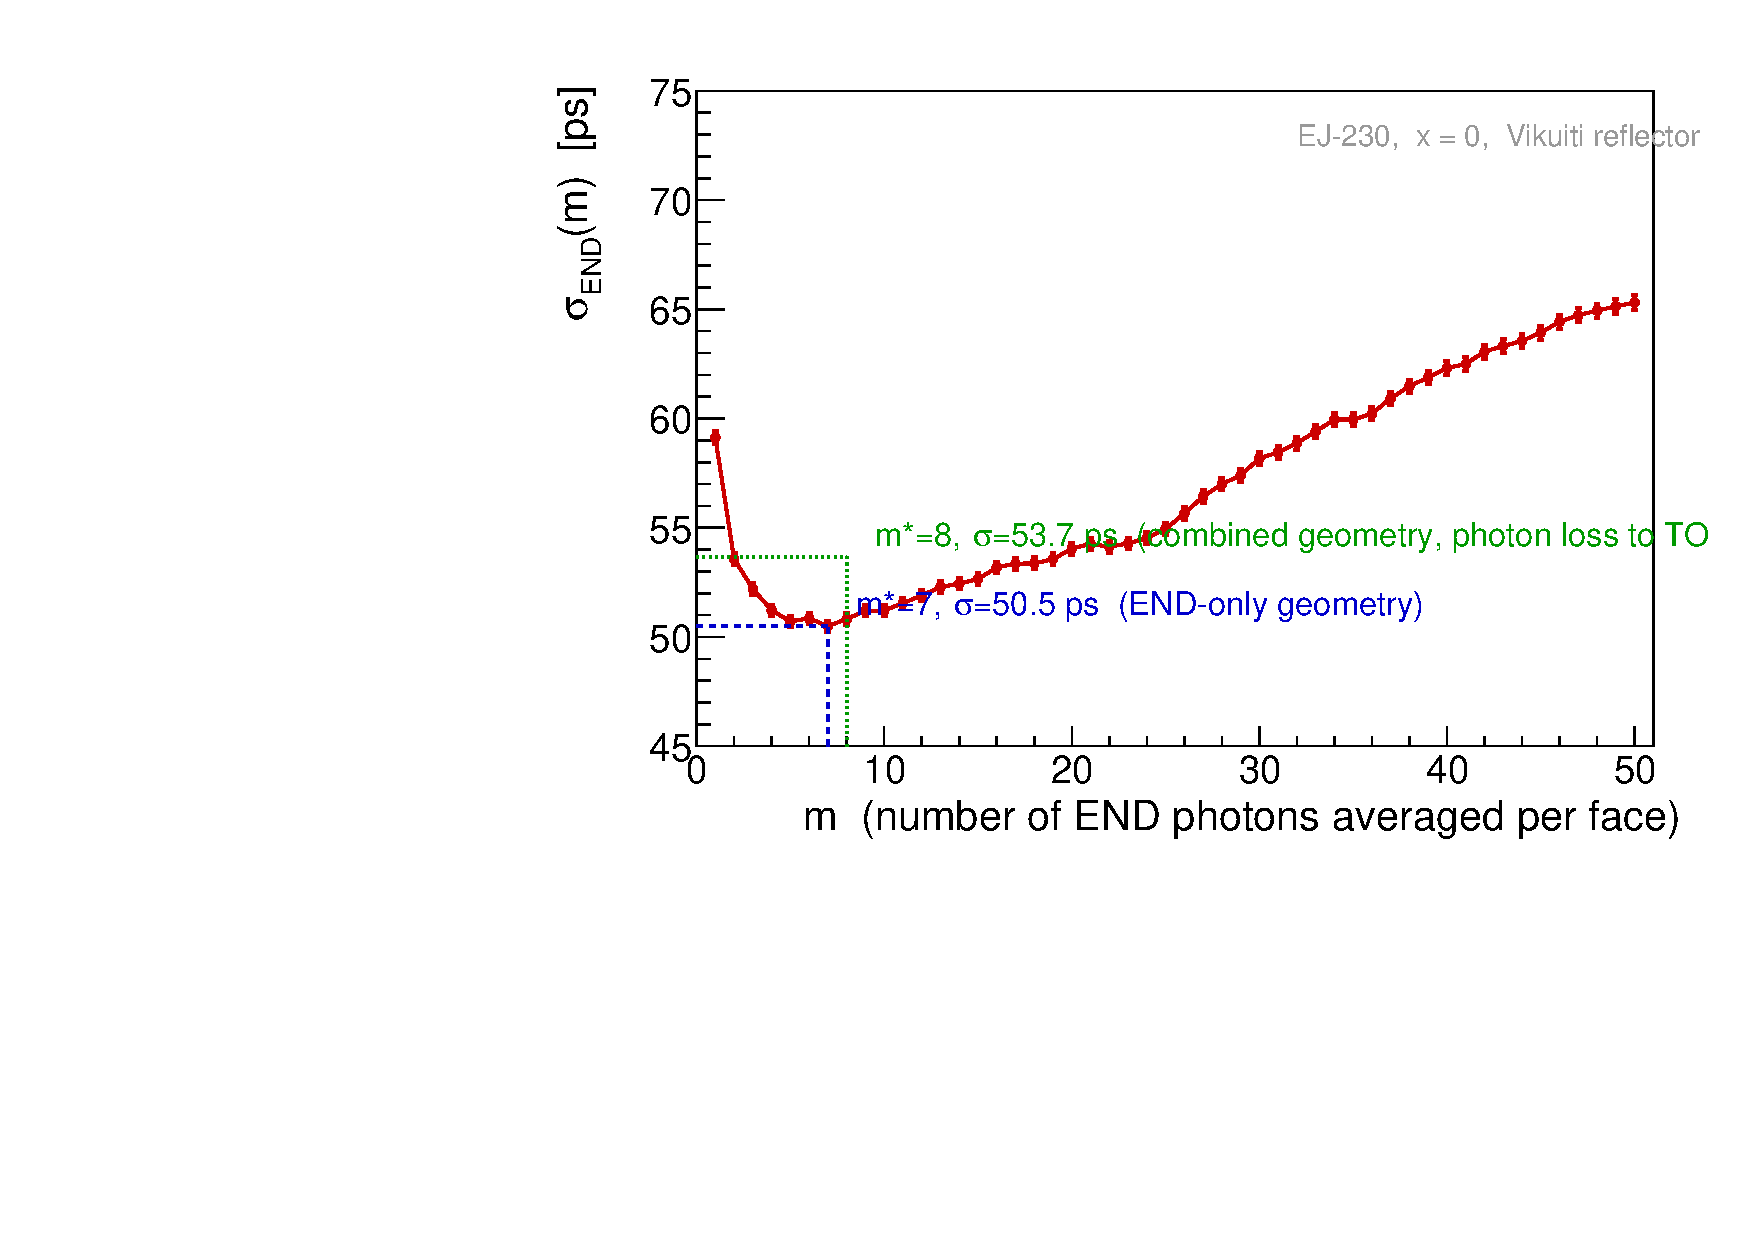
\includegraphics[width=\linewidth]{figs/fig_end_mscan.pdf}
\column{0.44\textwidth}
\begin{block}{$m$-average estimator}
\begin{equation*}
  \Tze = \frac{1}{2}\bigl(t_L^{(m)} + t_R^{(m)}\bigr),
  \quad
  t_{\alpha}^{(m)} = \frac{1}{m}\sum_{i=1}^m t_{\alpha,i}
\end{equation*}
\end{block}
\begin{itemize}\setlength\itemsep{3pt}
  \item Sort hits per event per face; take
    first $m$ arrival times
  \item Averaging over $m$ photons suppresses
    single-photon jitter
  \item Global optimum: $\mathbf{m=8}$
    (train/test at $x=0$)
  \item $\sEnd(x=0, m=8) = 53.7\ps$
  \item $\sEnd$ rises at bar ends as near-face
    photon pool shrinks
\end{itemize}
\end{columns}
\end{frame}

% ─────────────────────────────────────────────────────────────────────────────
\begin{frame}{TOP: $k$-th order statistic beats per-SiPM average}
\begin{columns}[c]
\column{0.52\textwidth}
\centering
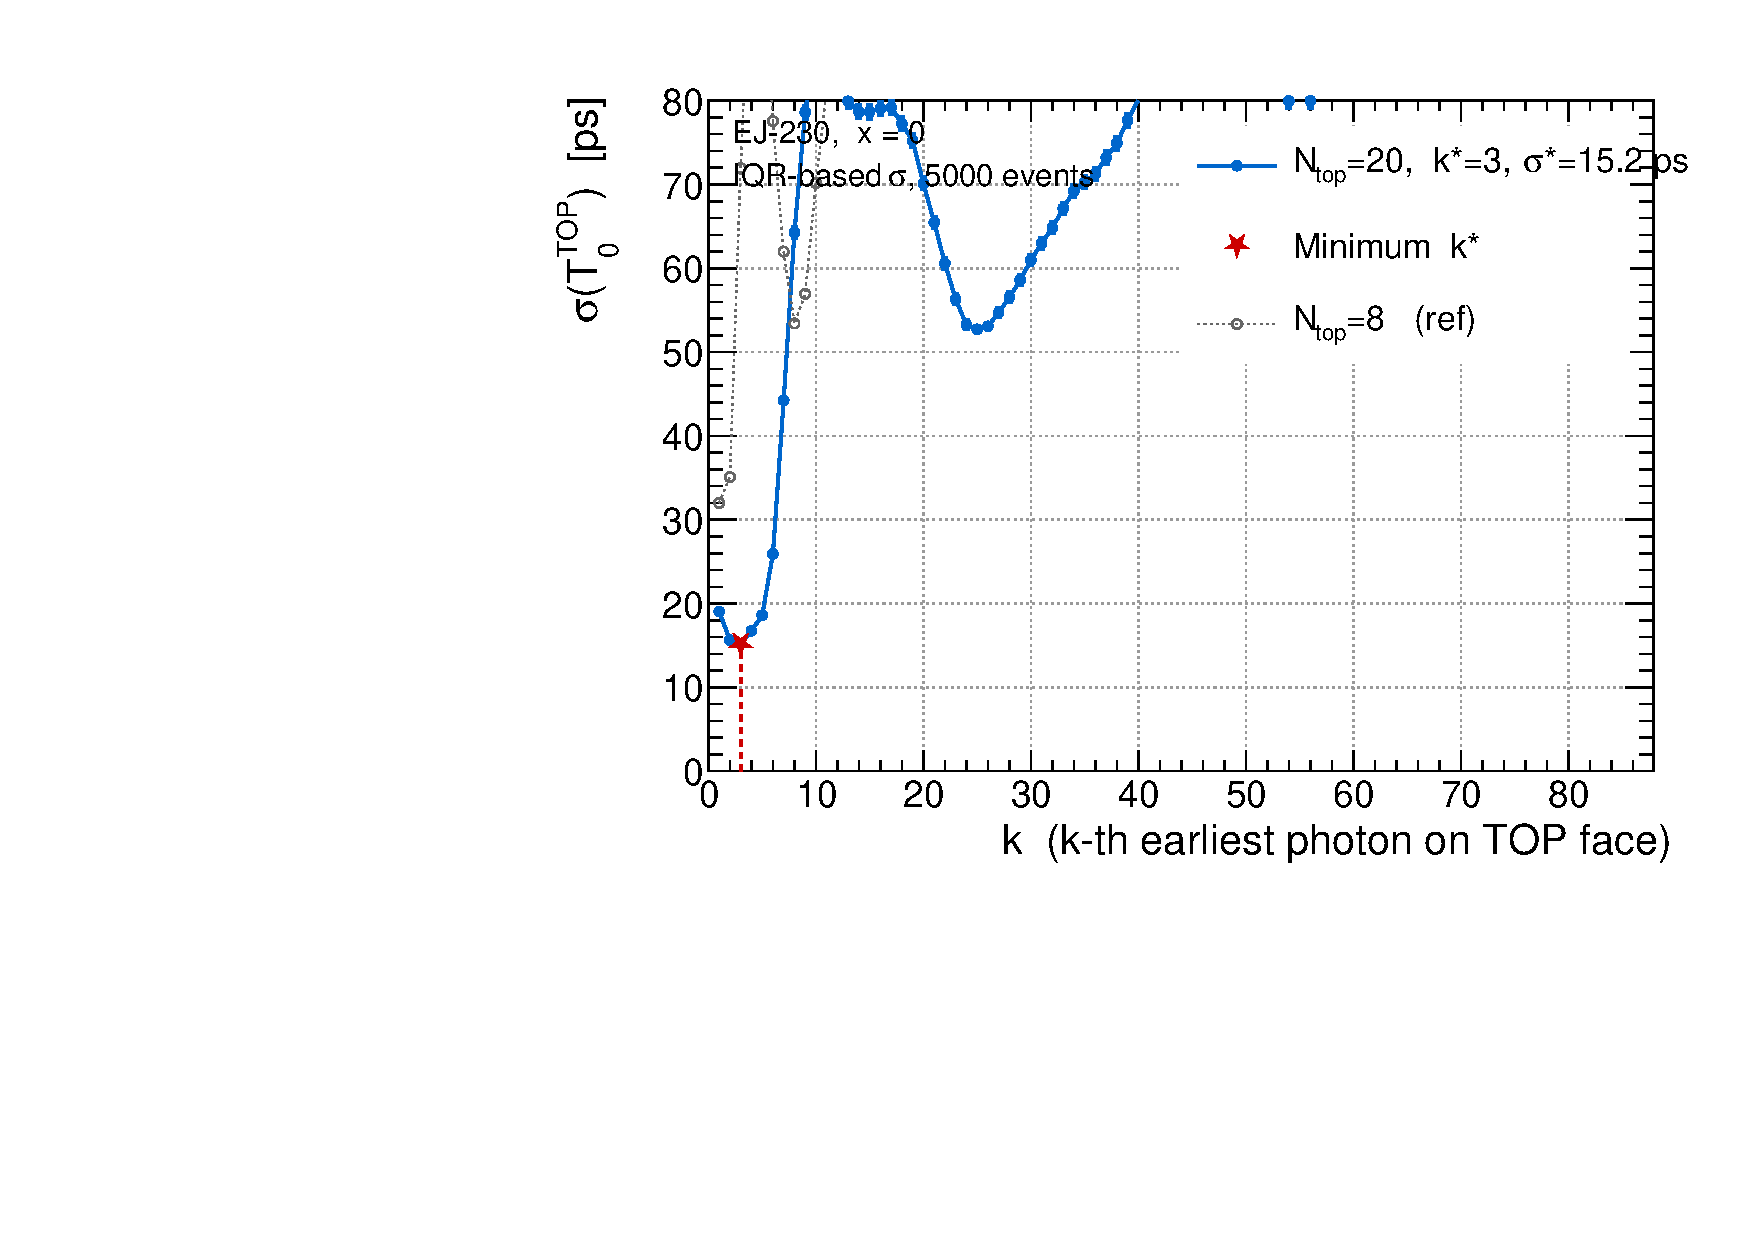
\includegraphics[width=\linewidth]{figs/fig1_kscan.pdf}
\column{0.44\textwidth}
\begin{block}{$k$-th order statistic (pooled)}
\begin{equation*}
  \Tzt = t_{(k)},\quad
  t_{(1)} \le t_{(2)} \le \cdots
\end{equation*}
Pool \emph{all} $\Ntop$ SiPMs; pick $k$-th earliest.
\end{block}
\begin{itemize}\setlength\itemsep{3pt}
  \item Global optimum: $\mathbf{k=3}$
    (train/test at $x=0$)
  \item $\sTop(x=0, k=3) = 15.2\ps$
  \item $3.6\times$ improvement over per-SiPM mean
  \item Low $k$ exploits first-photon statistics
    without dark-count sensitivity
  \item Insensitive to $x$: same photons reach
    TOP from all muon positions
\end{itemize}
\end{columns}
\end{frame}

% ─────────────────────────────────────────────────────────────────────────────
\section{BLUE Combination}

\begin{frame}{BLUE weights from ordinary covariance; $\sIQR$ is independent}
\begin{columns}[c]
\column{0.50\textwidth}
\begin{block}{BLUE combination}
\footnotesize
Given estimators $T_E$, $T_T$ with covariance matrix
\[
C = \begin{pmatrix} \mathrm{Var}(T_E) & \mathrm{Cov}(T_E,T_T) \\
\mathrm{Cov}(T_E,T_T) & \mathrm{Var}(T_T) \end{pmatrix}
\]
BLUE weight (ordinary Var/Cov):
\[
w_E = \frac{\mathrm{Var}(T_T) - \mathrm{Cov}}{%
  \mathrm{Var}(T_E)+\mathrm{Var}(T_T)-2\,\mathrm{Cov}},\quad
w_T = 1-w_E
\]
\[
T_0^{\mathrm{BLUE}} = w_E\,T_E + w_T\,T_T
\]
$\sIQR = (Q_{75}-Q_{25})/1.349$ is a \textbf{separate}
robust performance metric — not derived from $C$.
\end{block}
\column{0.46\textwidth}
\begin{block}{At $x=0$, $k=3$, $m=8$}
\small
\begin{tabular}{lr}
\toprule
Quantity & Value \\
\midrule
$\sEnd$ & $53.7\ps$ \\
$\sTop$ & $15.2\ps$ \\
$\sBlu$ & $\mathbf{15.0\ps}$ \\
$w_{\mathrm{END}}$ & $0.086$ \\
$w_{\mathrm{TOP}}$ & $0.914$ \\
$\rho(E,T)$ & $0.160$ \\
\bottomrule
\end{tabular}
\end{block}
\begin{alertblock}{Interpretation}
\small $w_{\mathrm{END}} \approx 0.09$ — when TOP has
$\sTop\approx15\ps$, END contributes only 9\% of the
weight. BLUE $\approx$ TOP at this configuration.
\end{alertblock}
\end{columns}
\end{frame}

% ─────────────────────────────────────────────────────────────────────────────
\section{Position Dependence}

\begin{frame}{Global estimator is deployable; oracle is a lower bound}
\begin{columns}[c]
\column{0.52\textwidth}
\centering
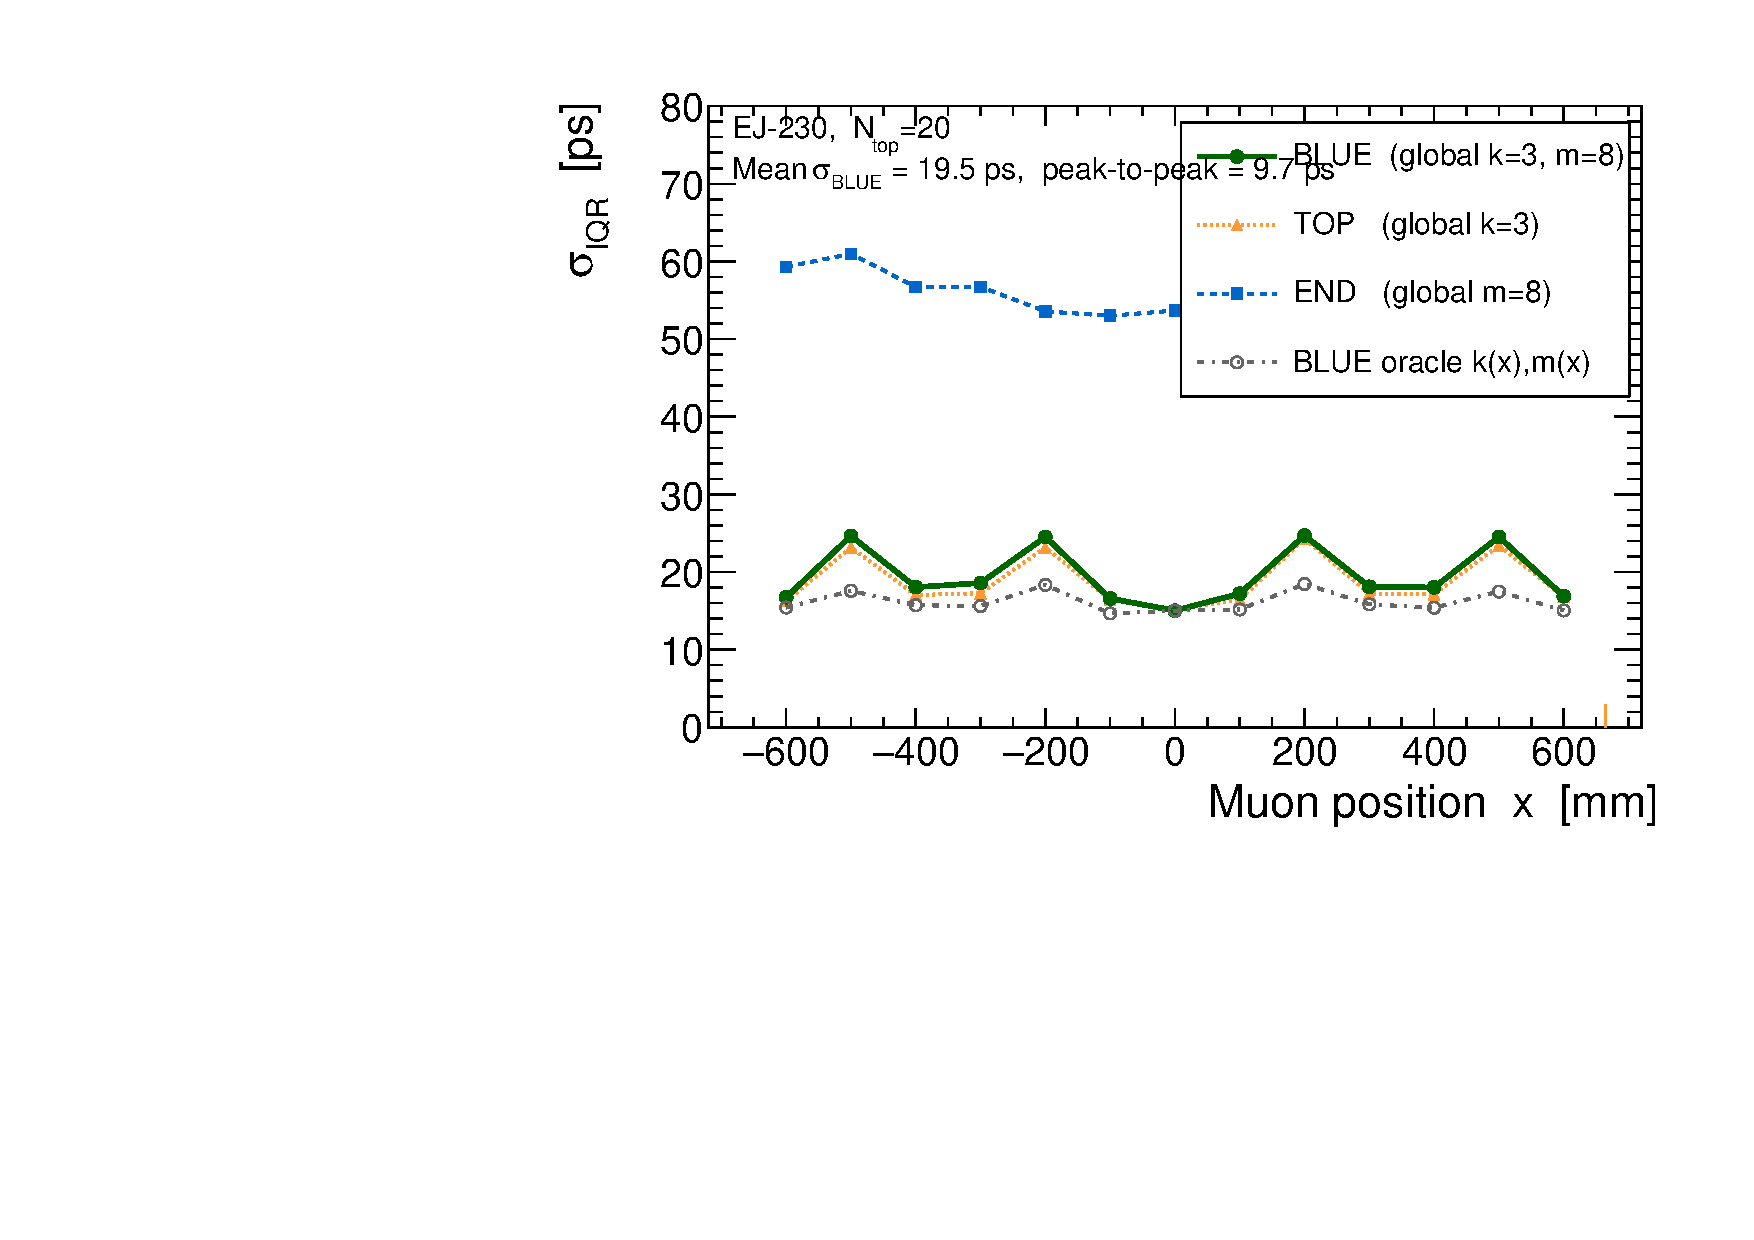
\includegraphics[width=\linewidth]{figs/v5_sigma_vs_x.pdf}
\column{0.44\textwidth}

\begin{block}{Two estimator classes}
\small
\textbf{Global} (k=3, m=8 fixed $\forall x$):\\
Deployable without per-position tuning\\[4pt]
\textbf{Oracle} (local opt.\ $k^*(x)$, $m^*(x)$):\\
Diagnostic lower bound — not deployable
\end{block}

\begin{block}{Results across $x \in [-600,+600]\mm$}
\scriptsize
\begin{tabular}{lrrr}
\toprule
 & Mean & Min & Max \\
\midrule
Global $\sBlu$ & 19.5 & 15.0 & 24.7 \\
Oracle $\sBlu$ & 16.1 & 14.7 & 18.5 \\
\bottomrule
\multicolumn{4}{l}{\small Units: ps}
\end{tabular}
\end{block}

\begin{itemize}\setlength\itemsep{2pt}
  \item Spikes at $x=\pm200,\pm500\mm$ where
    $k^*(x)=1$ but global uses $k=3$
  \item Oracle gap: $\sim3.4\ps$ (mean)
  \item Tick marks = TOP SiPM positions
\end{itemize}
\end{columns}
\end{frame}

% ─────────────────────────────────────────────────────────────────────────────
\begin{frame}{Global $\sBlu$ spikes at interstitial positions}
\begin{columns}[c]
\column{0.50\textwidth}
\footnotesize
\begin{tabular}{rrrrl}
\toprule
$x$ & $\sEnd$ & $\sTop$ & $\sBlu$ & note \\
\midrule
$-600$ & 59.3 & 16.3 & 16.7 & edge \\
$-500$ & 61.0 & 23.2 & 24.6 & \textcolor{cRef}{spike} \\
$-400$ & 56.7 & 17.0 & 18.1 & \\
$-300$ & 56.7 & 17.3 & 18.6 & \\
$-200$ & 53.6 & 23.2 & 24.5 & \textcolor{cRef}{spike} \\
$-100$ & 53.0 & 16.4 & 16.6 & \\
$\phantom{+}0$ & 53.7 & 15.2 & 15.0 & \\
$+100$ & 53.8 & 16.5 & 17.2 & \\
$+200$ & 55.0 & 24.3 & 24.7 & \textcolor{cRef}{spike} \\
$+300$ & 55.3 & 17.2 & 18.1 & \\
$+400$ & 57.6 & 17.1 & 18.0 & \\
$+500$ & 59.7 & 23.5 & 24.5 & \textcolor{cRef}{spike} \\
$+600$ & 61.0 & 16.8 & 16.9 & edge \\
\bottomrule
\multicolumn{5}{l}{\scriptsize Units: ps; global $k=3$, $m=8$}
\end{tabular}
\column{0.46\textwidth}
\begin{itemize}\setlength\itemsep{4pt}
  \item Spikes at $x=\pm200,\pm500\mm$: these lie
    between TOP SiPMs, so the $k=3$ photon
    arrives later than when $x$ is near a SiPM
  \item Oracle uses $k^*(x)=1$ at these positions,
    recovering $\sTop \approx 17$-$18\ps$
  \item No spike in END timing — it responds
    monotonically with distance
  \item Reducing $k$ globally (e.g.\ $k=1$) would
    help at spikes but hurt at SiPM positions
  \item Trade-off is fundamental to fixed-parameter
    deployment
\end{itemize}
\end{columns}
\end{frame}

% ─────────────────────────────────────────────────────────────────────────────
\section{$N_{\mathrm{TOP}}$ Scan}

\begin{frame}{More TOP SiPMs → better BLUE; returns diminish after $N=14$}
\begin{columns}[c]
\column{0.52\textwidth}
\centering
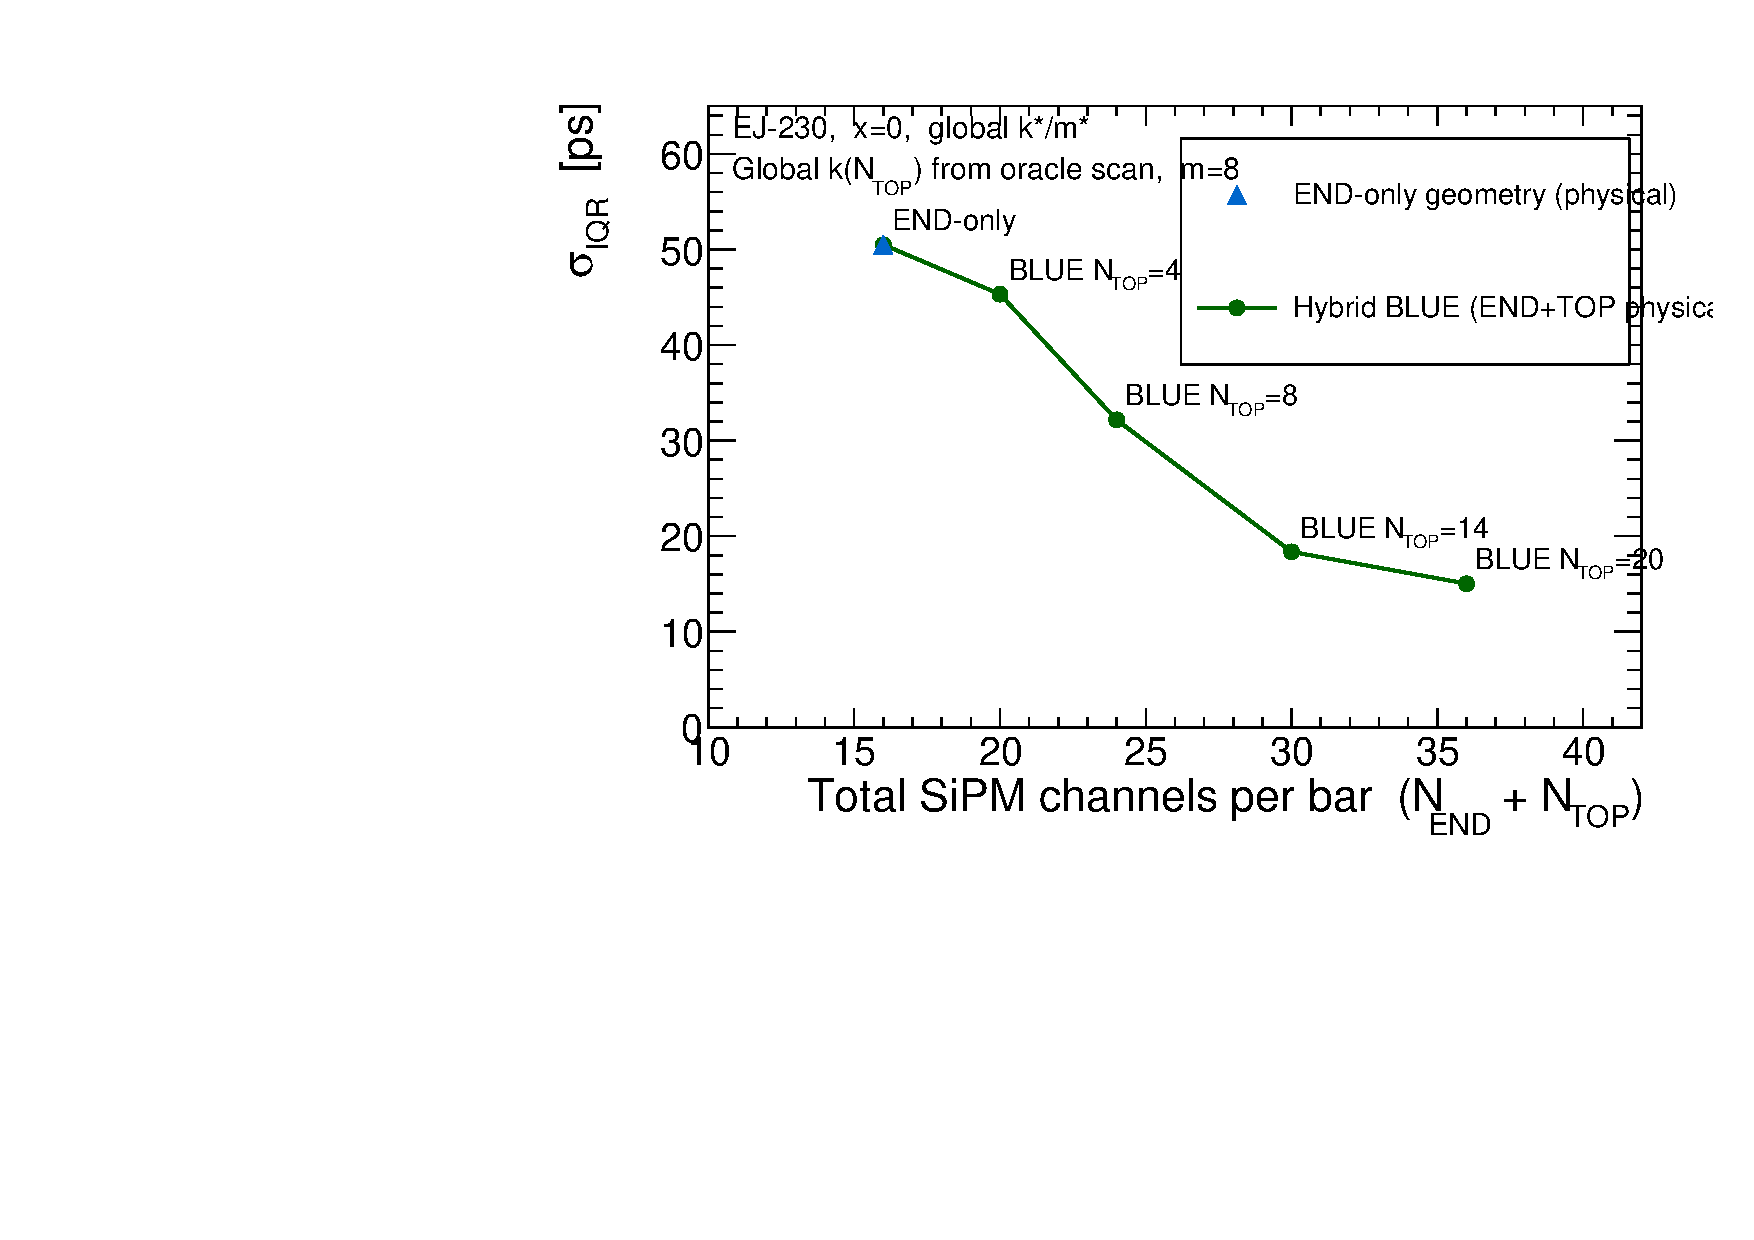
\includegraphics[width=\linewidth]{figs/v5_pareto.pdf}
\column{0.44\textwidth}
\begin{block}{Physical geometries, $x=0$}
\small
\begin{tabular}{ccccc}
\toprule
$\Ntop$ & $k^*$ & $\sTop$ & $\sBlu$ & $w_E$ \\
\midrule
4  & 1 & 78.2 & 45.3 & 0.77 \\
8  & 1 & 32.0 & 32.2 & 0.44 \\
14 & 2 & 18.7 & 18.4 & 0.17 \\
20 & 3 & 15.2 & 15.0 & 0.09 \\
\bottomrule
\multicolumn{5}{l}{\scriptsize ps; $m=8$ fixed; $k^*$ from oracle scan}
\end{tabular}
\end{block}
\begin{itemize}\setlength\itemsep{3pt}
  \item $\Ntop=4$: END dominates ($w_E=0.77$)
  \item $\Ntop=14$: $\sBlu\approx18\ps$, $3\times$
    fewer channels than $\Ntop=20$
  \item $\Ntop=20$: $\sBlu=15.0\ps$, END weight
    collapses to $9\%$
  \item $k^*$ grows with $\Ntop$: more SiPMs
    means more photons to pick from
\end{itemize}
\end{columns}
\end{frame}

% ─────────────────────────────────────────────────────────────────────────────
\section{TOP Position Measurement}

\begin{frame}{TOP centroid saturates at bar ends — END is better for position}
\begin{columns}[c]
\column{0.52\textwidth}
\centering
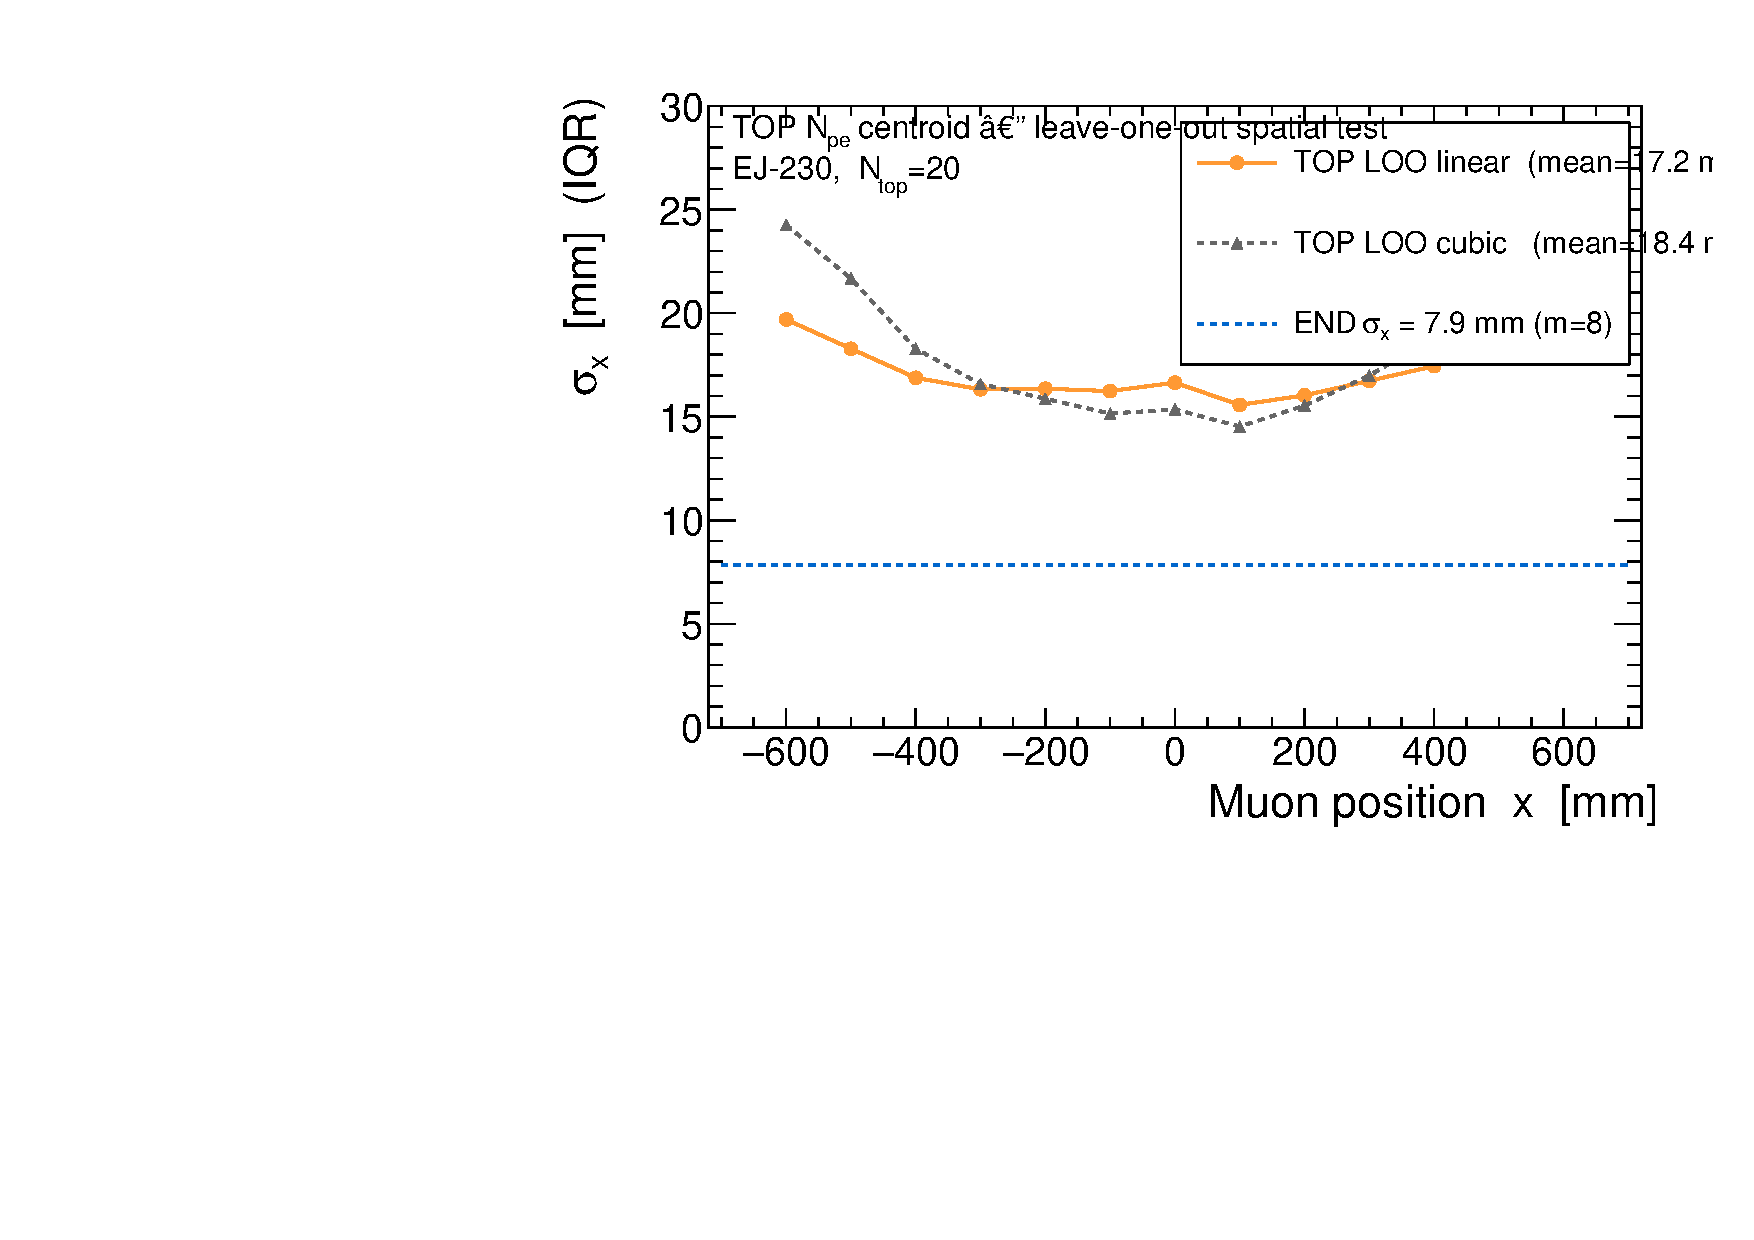
\includegraphics[width=\linewidth]{figs/v5_top_position_loo.pdf}
\column{0.44\textwidth}
\begin{block}{$N_{\mathrm{pe}}$-weighted centroid}
\[
x_c = \frac{\sum_i N_{\mathrm{pe},i}\,x_i^{\mathrm{SiPM}}}%
{\sum_i N_{\mathrm{pe},i}}
\]
\end{block}
\begin{itemize}\setlength\itemsep{3pt}
  \item SiPMs span $\pm664\mm$; centroid compressed to $\pm313\mm$ at bar edges
  \item LOO: train on 12 positions, predict 13th
  \item \textbf{Linear}: mean $\sigma_x=17.2\mm$,
    max $|\mathrm{bias}|=29\mm$ at ends
  \item \textbf{END} $\Delta t$ position:
    $\sigma_x=\mathbf{7.9\mm}$ (from $v_{\rm eff}$)
  \item END is $2\times$ better and has no edge bias
  \item TOP centroid still useful for tracking in
    a multi-bar system
\end{itemize}
\end{columns}
\end{frame}

% ─────────────────────────────────────────────────────────────────────────────
\section{Conclusions}

\begin{frame}{Conclusions}
\begin{columns}[c]
\column{0.50\textwidth}
\begin{block}{EJ-230 + END+TOP hybrid}
\begin{itemize}\setlength\itemsep{3pt}
  \item EJ-230: fastest scintillator
    ($\tau=1.5\ns$, att$=1200\mm$)
  \item Reflector: $R=0.95$ constant
    (Vikuiti ESR, dielectric-dielectric)
  \item $\veff = 177.6\mm/\mathrm{ns}$,
    $\chi^2/\mathrm{ndf}=1250/11$ — statistically
    significant nonlinearity (RMS$=14.5\ps$)
\end{itemize}
\end{block}

\begin{block}{Timing performance}
\begin{itemize}\setlength\itemsep{3pt}
  \item END ($m=8$): $\sEnd = 53.7\ps$ at $x=0$
  \item TOP ($k=3$, $\Ntop=20$): $\sTop = 15.2\ps$
  \item BLUE global: $\sBlu=15.0\ps$ at $x=0$,\\
    mean $= 19.5\ps$ across full bar
  \item Oracle: mean $16.1\ps$ — $3.4\ps$ gap
    shows cost of fixed parameters
\end{itemize}
\end{block}

\column{0.46\textwidth}
\begin{block}{$\Ntop$ trade-off}
\begin{itemize}\setlength\itemsep{3pt}
  \item $\Ntop=4$: $45.3\ps$ (END-dominated)
  \item $\Ntop=14$: $18.4\ps$ (3$\times$ fewer ch.)
  \item $\Ntop=20$: $15.0\ps$ (recommended)
\end{itemize}
\end{block}

\begin{block}{Position}
\begin{itemize}\setlength\itemsep{3pt}
  \item END $\Delta t$: $\sigma_x=7.9\mm$
  \item TOP centroid (LOO): $\sigma_x=17.2\mm$,
    large bias at edges — END preferred
\end{itemize}
\end{block}

\begin{alertblock}{Next steps}
\begin{itemize}\setlength\itemsep{2pt}
  \item Cubic correction for $\Delta t$ nonlinearity
  \item Systematic: dark counts, SiPM cross-talk
  \item Test on beam data
\end{itemize}
\end{alertblock}
\end{columns}
\end{frame}

% ─────────────────────────────────────────────────────────────────────────────
%  BACKUP SLIDES
% ─────────────────────────────────────────────────────────────────────────────
\appendix
\section*{Backup}

\begin{frame}{PDE: what 0.607 means}
\begin{columns}[c]
\column{0.50\textwidth}
\begin{block}{Recorded PDE in simulation}
\begin{itemize}\setlength\itemsep{4pt}
  \item The SiPM model applies a wavelength-dependent efficiency curve
  \item Each \emph{detected} photon carries its efficiency as the \texttt{pde} branch
  \item Mean over \textbf{detected photons}: $\langle\mathrm{PDE}\rangle = 0.607$
\end{itemize}
\end{block}
\begin{alertblock}{Selection bias}
This is \emph{not} the detection fraction.
High-PDE photons are over-represented because
they are more likely to be accepted. The
correct photon budget uses
$N_{\mathrm{detected}} / N_{\mathrm{emitted}}$.
\end{alertblock}
\column{0.46\textwidth}
\begin{block}{By face (x=0, EJ-230, $\Ntop=20$)}
\small
\begin{tabular}{lrr}
\toprule
Face & $\langle\mathrm{PDE}\rangle_{\mathrm{det}}$ & $\Npe$/ev \\
\midrule
END-L & 0.608 & 515 \\
END-R & 0.608 & 515 \\
TOP   & 0.606 & 1341 \\
\midrule
All   & 0.607 & — \\
\bottomrule
\end{tabular}
\end{block}
\begin{itemize}\setlength\itemsep{3pt}
  \item 11.85M detected hits at $x=0$
  \item TOP captures $\sim2.6\times$ more photons
    than each END face
  \item More photons support lower $k$ on TOP
\end{itemize}
\end{columns}
\end{frame}

% ─────────────────────────────────────────────────────────────────────────────
\begin{frame}{Reflector model: $R=0.95$ constant (not spectral)}
\begin{columns}[c]
\column{0.50\textwidth}
\begin{block}{Geant4 surface: \texttt{CreateBarSkinReflector()}}
\begin{itemize}\setlength\itemsep{3pt}
  \item Type: \texttt{dielectric\_dielectric}
  \item Model: \texttt{unified}
  \item Finish: \texttt{polished}
  \item Reflectivity: $R=0.95$ (constant,
    wavelength-independent)
\end{itemize}
\end{block}
\begin{itemize}\setlength\itemsep{3pt}
  \item Source: \texttt{src/Materials.cc},
    \texttt{CreateBarSkinReflector()}
  \item Lateral faces wrapped in air-gap + Mylar
    in the physical geometry
  \item \emph{Not} the full Vikuiti ESR spectral
    table — a conservative constant
\end{itemize}
\column{0.46\textwidth}
\begin{block}{SiPM surface: wavelength-dependent PDE}
\begin{itemize}\setlength\itemsep{3pt}
  \item \texttt{SiPMModel::LoadPDECurve()}
  \item Applied at each photon absorption step
  \item Results in $\langle\mathrm{PDE}\rangle=0.607$
    over detected population (selection-biased)
\end{itemize}
\end{block}
\begin{alertblock}{Implication}
The reflector is a constant, not the Vikuiti
spectral curve. Real Vikuiti $R\sim0.98$–$0.99$
would yield more photons and better timing.
\end{alertblock}
\end{columns}
\end{frame}

% ─────────────────────────────────────────────────────────────────────────────
\begin{frame}{Oracle $k^*(x)$ and $m^*(x)$ vary across positions}
\begin{columns}[c]
\column{0.48\textwidth}
\footnotesize
\begin{tabular}{rrrrrr}
\toprule
$x$ & $k^*$ & $\sTop^*$ & $m^*$ & $\sEnd^*$ & $\sBlu^*$ \\
\midrule
$-600$ & 2 & 15.4 & 10 & 59.0 & 15.4 \\
$-500$ & 1 & 17.8 & 11 & 60.1 & 17.6 \\
$-400$ & 2 & 15.9 & \phantom{1}5 & 55.4 & 15.7 \\
$-300$ & 2 & 16.0 & \phantom{1}6 & 56.3 & 15.6 \\
$-200$ & 2 & 17.6 & \phantom{1}8 & 53.6 & 18.3 \\
$-100$ & 2 & 14.9 & \phantom{1}6 & 52.8 & 14.7 \\
$\phantom{+}0$ & 3 & 15.2 & \phantom{1}8 & 53.7 & 15.0 \\
$+100$ & 2 & 15.6 & \phantom{1}5 & 53.1 & 15.2 \\
$+200$ & 2 & 18.2 & 10 & 54.5 & 18.5 \\
$+300$ & 2 & 15.8 & \phantom{1}7 & 54.9 & 15.8 \\
$+400$ & 2 & 15.8 & \phantom{1}5 & 57.4 & 15.4 \\
$+500$ & 1 & 17.5 & \phantom{1}5 & 58.8 & 17.5 \\
$+600$ & 2 & 15.3 & \phantom{1}5 & 60.9 & 15.1 \\
\bottomrule
\multicolumn{6}{l}{\scriptsize ps; oracle = same-sample optimum}
\end{tabular}
\column{0.48\textwidth}
\begin{itemize}\setlength\itemsep{4pt}
  \item Oracle $k^*=1$ at $x=\pm500\mm$
    (interstitial, few early photons in TOP)
  \item Oracle $k^*=3$ only at $x=0$ where
    global = oracle
  \item Global $k=3$ is not optimal at most
    positions — hence the spikes in global $\sBlu$
  \item Oracle $m^*$ ranges 5–11: END optimal $m$
    also varies with photon count
  \item Oracle diagnostic confirms the fundamental
    limit $\sBlu \approx 15\ps$ is achievable
    at all positions (with position-dependent tuning)
\end{itemize}
\end{columns}
\end{frame}

% ─────────────────────────────────────────────────────────────────────────────
\begin{frame}{Estimator train/test validation at $x=0$}
\begin{columns}[c]
\column{0.50\textwidth}
\begin{block}{50/50 split, $x=0$, EJ-230, $\Ntop=20$}
\small
\begin{tabular}{lrr}
\toprule
Estimator & Train & Test \\
\midrule
$m^*$       & 7      & —     \\
$k^*$       & 3      & —     \\
$\sEnd$ [ps] & 53.7  & 54.0  \\
$\sTop$ [ps] & 15.6  & 15.0  \\
$\sBlu$ [ps] & (cross) & 14.8\\
$w_{\mathrm{END}}$ & — & 0.020 \\
$\rho$      & — & 0.141 \\
\bottomrule
\end{tabular}
\end{block}
\begin{itemize}\setlength\itemsep{3pt}
  \item Optimal $m^*=7$ (train); global uses $m=8$
  \item At $x=0$: global and oracle agree —
    $k=3$, $m=8$ is near-optimal
\end{itemize}
\column{0.46\textwidth}
\begin{block}{Gaussian fit at $x=0$ (oracle $k=3$, $m=8$)}
\small
\begin{tabular}{lrrl}
\toprule
Est. & $\sIQR$ & $\sigma_G$ & $\chi^2$/ndf \\
\midrule
END  & 53.7 & 53.3 & 65.8/52 \\
TOP  & 15.2 & 14.8 & 62.0/53 \\
BLUE & 15.2 & 14.6 & 83.6/53 \\
\bottomrule
\multicolumn{4}{l}{\scriptsize ps; BLUE non-Gaussian ($p=0.005$)}
\end{tabular}
\end{block}
\begin{itemize}\setlength\itemsep{3pt}
  \item END and TOP are consistent with Gaussian
  \item BLUE slightly non-Gaussian ($p=0.005$)
    due to the nonlinear weight combination
  \item $\sIQR$ is the robust metric; Gaussian
    $\sigma$ shown for comparison only
\end{itemize}
\end{columns}
\end{frame}

% ─────────────────────────────────────────────────────────────────────────────
\begin{frame}{TOP $N_{\mathrm{pe}}$ centroid — saturation at bar ends}
\begin{columns}[c]
\column{0.50\textwidth}
\begin{itemize}\setlength\itemsep{4pt}
  \item TOP SiPMs span $x \in [-664, +664]\mm$
    (spacing $\approx70\mm$)
  \item Centroid is bounded by the SiPM range
  \item At $x=\pm600\mm$ muon, median centroid
    is only $\pm313\mm$ — compression by $2\times$
  \item Linear calibration has maximum
    $|\mathrm{bias}|=29\mm$ at bar edges
  \item Cubic calibration reduces bias but
    does not improve $\sigma_x$
  \item Both are worse than END $\Delta t$
    ($\sigma_x=7.9\mm$) at all positions
\end{itemize}
\column{0.46\textwidth}
\begin{block}{LOO centroid medians}
\scriptsize
\begin{tabular}{rrrr}
\toprule
$x_{\rm true}$ & $\bar x_c$ & $\sigma_c$ [mm] \\
\midrule
$-600$ & $-313$ & 10.7 \\
$-500$ & $-273$ & 9.9 \\
$-400$ & $-218$ & 9.1 \\
$-300$ & $-168$ & 8.8 \\
$-200$ & $-121$ & 8.8 \\
$-100$ & $-58$ & 8.8 \\
$\phantom{+}0$ & $+0$ & 9.0 \\
$+100$ & $+58$ & 8.4 \\
$+200$ & $+120$ & 8.6 \\
$+300$ & $+168$ & 9.0 \\
$+400$ & $+218$ & 9.4 \\
$+500$ & $+273$ & 9.9 \\
$+600$ & $+313$ & 10.5 \\
\bottomrule
\end{tabular}
\end{block}
\end{columns}
\end{frame}

\end{document}
